\documentclass[11pt]{article}
\usepackage{geometry}
\geometry{a4paper, left=25mm, right=25mm, top=25mm, bottom=30mm}

\usepackage{amsmath}
\usepackage{graphicx}
\usepackage{booktabs}
\usepackage{siunitx}
\usepackage{microtype}
\usepackage{parskip}
\usepackage{hyperref}
\usepackage{xcolor}
\usepackage{listings}
\usepackage{titling}
\usepackage{mdframed}
\usepackage{changepage}

\definecolor{codegreen}{rgb}{0.33, 0.71, 0.36}
\definecolor{codegray}{rgb}{0.5, 0.5, 0.5}
\definecolor{codepurple}{rgb}{0.58, 0, 0.82}
\definecolor{backcolour}{rgb}{0.95, 0.95, 0.92}
\definecolor{codeblue}{rgb}{0.25,0.5,0.8}

\lstset{
    backgroundcolor=\color{backcolour},   
    commentstyle=\color{codegreen},
    keywordstyle=\color{codeblue},
    numberstyle=\tiny\color{codegray},
    stringstyle=\color{codepurple},
    basicstyle=\ttfamily\footnotesize,
    breakatwhitespace=false,         
    breaklines=true,                 
    captionpos=b,                    
    keepspaces=true,                 
    numbers=left,                    
    numbersep=5pt,                  
    showspaces=false,                
    showstringspaces=false,
    showtabs=false,                  
    tabsize=2,
    language=Python
}

\title{}
\author{Sebastian M.D.}
\date{March 2024}

\mdfdefinestyle{leftLine}{
    linecolor=black,
    outerlinewidth=1pt,
    bottomline=false,
    topline=false,
    rightline=false,
    leftmargin=10pt,
    rightmargin=10pt,
    skipabove=0pt,
    skipbelow=0pt,
    innertopmargin=0pt,
    innerbottommargin=0pt,
}

\pretitle{%
  \begin{center}
  \begin{mdframed}[style=leftLine]
    Supervisor: Thomas Lennartson
    
    Program: Natural Sciences Program
    
    School: Procivitas Privata Gymnasium Malmö 
    \end{mdframed} 
    \vspace{3em}
  \huge
Which Neural Network Architecture is Optimal for Predicting Chaotic Dynamics? \\
\vspace{1em}
\small
\begin{adjustwidth}{2cm}{2cm}
A comparative study between RNN, Transformers and Echo State Networks regarding their capacity to predict the Lorenz 63 system.
\end{adjustwidth}
\vspace{14em}
\begin{figure}[h]
\centering
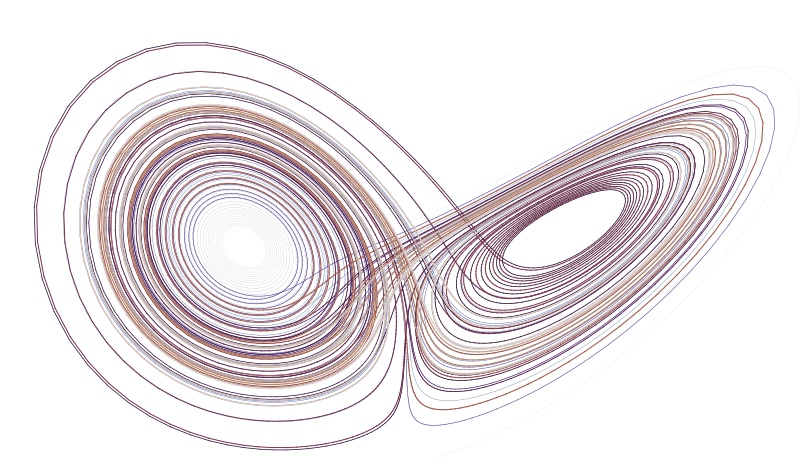
\includegraphics[width=0.8\textwidth]{title_page_image.jpeg}
\end{figure}

}
\posttitle{\end{center}}



\preauthor{\vfill\begin{center}\large}
\postauthor{\end{center}}

\predate{\begin{center}\large}
\postdate{\end{center}}

\begin{document}


\maketitle
\thispagestyle{empty} % Removes the page number

\newpage
\null\vspace*{\stretch{1}}
\begin{abstract}
    % Should be complete overview of purpose, method, results and conclusion, needs to be rewritten
\noindent This paper explores the application of neural networks in predicting the trajectory of the Lorenz 63 system, a set of differential equations that showcase chaotic behavior. The Lorenz System was originally stipulated by Edward N. Lorenz in 1963 as a mathematical model for atmospheric convection and is commonly used as a toy problem to explore chaos theory. Traditional numerical methods such as the Runga Kutta 4th order method can be used to solve and predict the system's behavior. This study explores the use of neural networks as an alternative approach to predict chaos. The methodology involves training a neural network on a dataset generated from the Lorenz system via the RK4 method. By using a small step size and high computational resources, the network can generalize patterns and possibly later on efficiently predict the system's future state with different initial conditions. This paper aims to test the RNN LSTM, Transformers, and RC-ESN network architectures. RNN and Transformer architectures are known for their ability to handle sequential data, while RC-ESN is known for its ability to capture chaotic systems. The results of the study will be compared to the RK4 method to determine if the neural networks could surpass it with a greater prediction horizon given similar computational resources.
\end{abstract}
\vspace*{\stretch{2}}
\newpage


\tableofcontents
\newpage

\section{Introduction}
A chaotic system is a dynamical system that is highly sensitive to initial conditions, leading to long-term unpredictability despite its deterministic nature. Chaotic systems are found in many natural phenomena, such as weather, water flows, and planetary orbits. Traditionally chaotic systems have been modeled using numerical methods, however papers such as \cite{npg-27-373-2020} have tried to apply neural network models instead. Neural networks are computing systems that mimic the brain to learn from data and recognize patterns without explicit instructions. Results have shown that neural networks, specifically echo state networks, can be promising in capturing chaotic dynamics. The goal of this study is to further explore the application of neural networks by also testing out the Transformers architecture as introduced by Google in their research paper \cite{DBLP:journals/corr/VaswaniSPUJGKP17} and compare it to the RNN and ESN architectures. The networks will be judged on their mean squared error over time and their ability to capture the Lorenz 63 system's chaotic patterns. The objective is to detemine which of these architecture prove most effective in predicting chaotic systems.
\section{Theory}

\subsection{The Lorenz System}

The original Lorenz system is a set of three differential equations. It is one of the earliest and most studied examples of systems that exhibit chaotic behavior. It is defined by the following equations:

\begin{align}
\frac{dx}{dt} &= \sigma(y - x) \\
\frac{dy}{dt} &= x(\rho - z) - y \\
\frac{dz}{dt} &= xy - \beta z
\end{align}

where $x$, $y$, and $z$ make up the system's positional state with respect to time $t$, and $\sigma$, $\rho$, and $\beta$ are parameters. Typically, the values $\sigma = 10$, $\rho = 28$, and $\beta = \frac{8}{3}$ are used.

The Lorenz system is known for its butterfly-shaped attractor, which is a set of two points the systems tends to evolve around, regardless of the starting conditions. The attractor is visualized in Figure \ref{fig:lorenz_attractor}.

\begin{figure}[h]
\centering
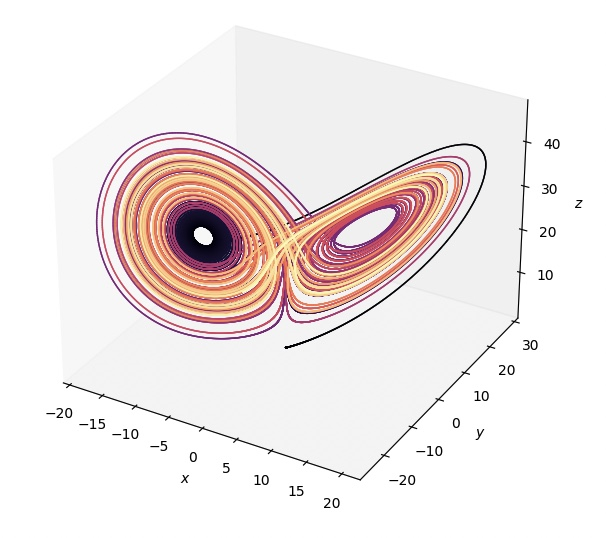
\includegraphics[width=0.3\textwidth]{lorenz_attractor.jpeg}
\caption{The Lorenz attractor for $\sigma = 10$, $\rho = 28$, and $\beta = \frac{8}{3}$. Generated with RK4 method for 100 time units}
\label{fig:lorenz_attractor}
\end{figure}

\subsection{Neural Networks}

Neural networks are a type of machine learning model that are inspired by the structure of the human brain. They are composed of layers with interconnected nodes, which represent neurons, that process input data and produce an output. These nodes are usually connected to each other with linear transformations called weights (\(W\)) and biases (\(b\)). The weights and biases are the parameters of the network that initially are randomly initialized and are optimized during the training process. \\

At the heart of neural networks is the feedforward computation that passes the data from one layer \(x\) to the next \(y\) as follows:

\[ y = f(Wx + b) \]

where \(y\) is the output, \(W\) is the weights matrix, \(x\) is the input vector, \(b\) is the bias vector, and \(f\) is the activation function, typically the ReLU(rectified linear unit) function is used. the ReLU function is defined as:

\[ \text{ReLU}(z) = \max(0, z) \]

Which maps all positive inputs to themselves while negative inputs are mapped to zero. The ReLU activation function introduces non-linearity to the model, which is critical for capturing complex behavior. Another popular activation function is the hyperbolic tangent or tanh, which squashes the input values to be within the range \(-1\) and \(1\):

\[
\text{tanh}(z) = \frac{e^{z} - e^{-z}}{e^{z} + e^{-z}}
\]

This allows tanh to output values that have mean zero, which can make learning for the subsequent layers slightly easier. Another activation function commonly used for the output layer is the sigmoid function. The sigmoid function maps the input values to a range between \(0\) and \(1\), interpreted as probabilities:

\[
\sigma(z) = \frac{1}{1 + e^{-z}}
\]

Due to its shape, the sigmoid function is suitable for binary outputs and is useful when a probabilistic interpretation is desired for the output neuron. However, for multiclass classification tasks, the softmax activation function is commonly used instead. It maps the input vector to a probability distribution:

\[
\text{softmax}(z_i) = \frac{e^{z_i}}{\sum_{j=1}^{K} e^{z_j}}
\]

The softmax function ensures that the sum of the probabilities of all classes is \(1\), which is great for a probabilistic interpretation.

Given a predicted value \(\hat{y}_i\) and a true value \(y_i\) a cost function is used to measure the degree of error in the prediction. Commonly used for regression-based tasks is the mean squared error (MSE) function, which is defined by:

\[ C = \frac{1}{2n} \sum_{i=1}^{n} (y_i - \hat{y}_i)^2 \]

where \(C\) is the cost, \(n\) is the number of samples, \(y_i\) is the true value, and \(\hat{y}_i\) is the predicted value.

During the training process, optimization strategies such as stochastic gradient descent (SGD) are used. The gradient of the cost function is computed with respect to the weights in a process called backpropagation, and is used to adjust the weights in the direction that minimizes the cost:

\[ W_{\text{new}} = W_{\text{old}} - \eta \nabla C \]

where \(W_{\text{new}}\) and \(W_{\text{old}}\) are the values of the weights after and before the update, respectively, \(\nabla C\) is the gradient of the cost function with respect to the weights, and \(\eta\) is the learning rate.

Via processes like SGD, the network can compute a gradient to slowly shift the parameters and minimize the error of the network's predictions. Over time the network can generalize and learn the underlying patterns of the data to make accurate predictions on unseen data.

\subsection{RNNs}
A Recurrent Neural Network (RNN) is a type of neural network architecture designed to recognize patterns in sequential data. What makes the RNN architecture special is that it's composed of a train of nodes, called cells, each connected to the next, where all the cells share the same trainable weights and biases. Each node in the train has it's own hidden state that is used when computing the next ouput. When the input vector is fed to the first cell of the train, it creates an output and then the hidden state is updated and passed along to the next node. The hidden state makes it so the next cell can 'remember' the previous data inputed. The RNN is governed by these equations:

\begin{equation}
h^{(t)} = \tanh(Wh^{(t-1)} + Ux^{(t)} + b_h)
\end{equation}

\begin{equation}
y^{(t)} = \text{softmax}(Vh^{(t)} + b_y)
\end{equation}

Here \(h^{(t)}\) is the hiddens state at timestep $t$, and \(y^{(t)}\) the equivalent output at that timestep. The weights $W$, $U$ and $V$ and the biases $b_h$ and $b_y$ are trainable parameters of the network and they are the same for all nodes. These equations highlight the recurrent nature of the RNN, as the computation of the hidden state at time $t$ depends on the previous state at $t-1$. This is what allows the network to maintain a form of memory over time. See Figure 2 for a visual representation of the RNN architecture, where $o^{(t)}$ represents $y^{(t)}$ before softmax

\begin{figure}[h]
\centering
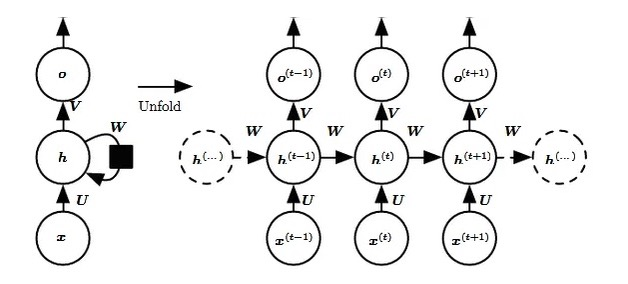
\includegraphics[width=0.8\textwidth]{rnn_diagram.jpeg}
\caption{https://www.deeplearningbook.org/contents/rnn.html}
\end{figure}

However, RNNs have a significant limitation in that they often struggle to learn long term dependencies, since during backpropgation, the gradients are propagated through the same weights matrix multiple times, which especially when dealing with long sequences can lead to the vanishing and exploding gradient problem where the gradients either becomes extremely small or extremely big. Long Short-Term Memory (LSTM) networks  aim to solve this problem. The LSTM network is a modification of the RNN that introduces a second hidden state, called the cell state, which is updated differently from the traditional hidden state. It is governed by these equations:

\begin{equation} a^{(t)} = Wh^{(t-1)} + Ux^{(t)} + b_h\end{equation}

Now $a^{(t)}$ is used to compute four gates, $i$, $f$, $o$, and $g$ with different biases and activation functions:

\begin{equation} i^{(t)} = \sigma(a^{(t)} + b_i) \end{equation}

\begin{equation} f^{(t)} = \sigma(a^{(t)} + b_f) \end{equation}

\begin{equation} o^{(t)} = \sigma(a^{(t)} + b_o) \end{equation}

\begin{equation} g^{(t)} = \tanh(a^{(t)} + b_g) \end{equation}

The gates are used to compute the next cell state, where the $f$ gate decides how much to 'remember' or 'forget' from the previous cell state, and the $i$ and $g$ gate together decide how much new information to write.

\begin{equation} C^{(t)} = f^{(t)} \odot C^{(t-1)} + i^{(t)} \odot g^{(t)} \end{equation}

The $o$ gate then detemines how much of the cell state to output to the next hidden state.

\begin{equation} h^{(t)} = o^{(t)} \odot \tanh(C^{(t)}) \end{equation}

Usually the output vector equals the hidden state in a LSTM.

\begin{equation} y^{(t)} = h^{(t)} \end{equation}

\begin{figure}[h]
\centering
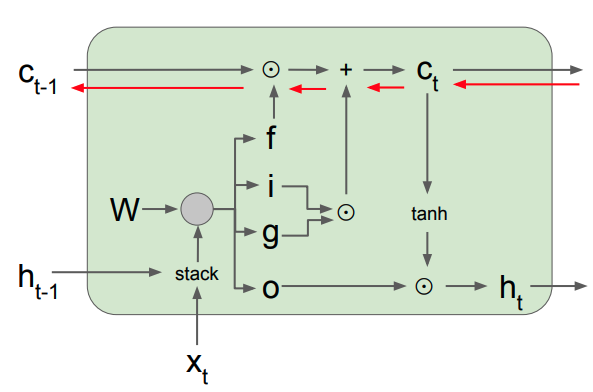
\includegraphics[width=0.6\textwidth]{lstm_diagram.png}
\caption{http://cs231n.stanford.edu/slides/2017/cs231n\_2017\_lecture10.pdf}
\end{figure}

Figure 3 showcases an LSTM cell, notice the red arrows which show the gradient flow. Because the hadamard product is used instead of matrix multiplication and the gates can vary between cells, gradient flow becomes more stable, which allows the network to learn long-term dependencies without an exploding or vanishing gradient.
\subsection{Transformers}

Transformers is a type of neural network architecture that was introduced in the paper "Attention is alll you need" \cite{DBLP:journals/corr/VaswaniSPUJGKP17}. Unlike RNNs, Transformers do not process the data in sequence, instead, they process the entire sequence at once. Transformers transform the data into an embedding layer where the positions are encoded into the data vectors themselves which allows for parallelization.

The key element in Transformers is the self-attention mechanism. In self-attention, each token in the input sequence is transformed with trainable weights into three vectors, a query $Q$, a key $K$ and a value $V$ vector. The query vector represents what a given token is looking for, the key vector what the token offers, whilst the value vector is the information the token contains.

$$\text{Attention}(Q, K , V) = \text{softmax}(\frac{QK^T}{\sqrt{d_k}})V$$

The self-attention mechanism takes the dot product between the keys and queries of the tokens, divides it by the square root of the key dimension(to prevent too small gradients) and then applies softmax to create a weights matrix. The weights matrix is used to determine how much each token in the sequence should contribute to the value vector of another token. For example, let the tokens be words in a sentence. In the sentence "The cat sat on the mat", the word "cat" would have a high affinity for the word "mat"(a query vector looking for the object of the sentence) and a low affinity for the word "the". This mechanism allows the network to learn the relationships between the tokens in the sequence.

The self attention mechanism is usually applied multiple times on the same tokens in parallell. This is called multi-head attention. Each 'head' has its own trainable transformations to look for different things in the tokens. The results are then concatenated and then aggregated through a trainable transformation to create the final ouput of the multi-head layer.

\begin{figure}[h]
\centering
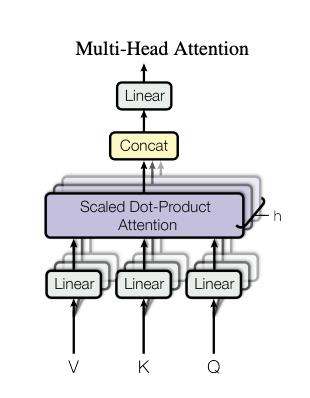
\includegraphics[width=0.3\textwidth]{multi-head.png}
\caption{Taken from "All you need is attention" by Google. }
\end{figure}

The multi-head layer is paired with a position-wise feed-forward layer. The feed-forward layer applies two trainable linear transformations with a ReLU activation in between. The feed forward layer makes it so the network can learn more complex representations of the data. The multi-head layer and feed-forward layer is usually repeated in blocks to form the transformer network. Between the layers goes a residual conection called layer normalization. Each time a multi-head or feed-forward layer has made a computation the result is added to the residual connection. This makes the gradient flow more stable.

\begin{figure}[h]
\centering
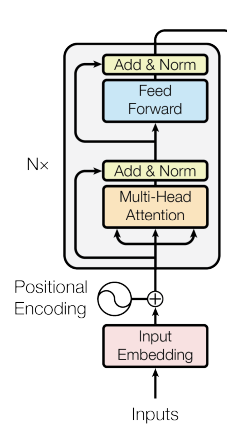
\includegraphics[width=0.3\textwidth]{transformer-basic.png}
\caption{Basic Transformers architecture, taken from "All you need is attention" by Google. }
\end{figure}

\subsection{Reservoir Computing and Echo State Networks}
Reservoir Computing (RC) is a variant of RNNs that has proven particularly effective in predicting chaotic systems. The fundamental principle behind reservoir computing is that only a part of the network is trained, while the rest of the network, the "reservoir" remains unchanged during training. This approach significantly reduces the computational cost of training RNNs and overcomes some of the issues related to gradient-based learning in traditional RNNs, such as vanishing and exploding gradients.

Echo State Networks (ESNs) are a particularly well-known implementation of reservoir computing. ESNs consist of a sparsely connected and randomly reservoir. The reservoir serves to project the input into a higher-dimensional space where the different parts of the input sequence become more linearly separable. Training only occurs in a readout layer, which is typically a linear model that is adjusted to map the reservoir states to the desired output.

\begin{figure}[h] 
\centering 
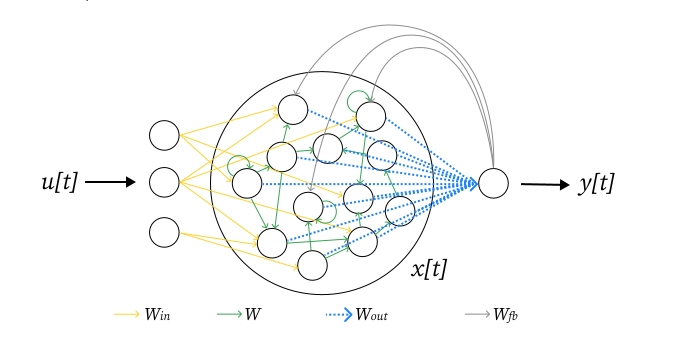
\includegraphics[width=0.8\textwidth]{echo_diagram.png} 
\caption{rservoirpy user guide docs}
\end{figure}

The key properties of an ESN are its dynamical richness and memory capacity, enabling it to process time-dependent information effectively. Reservoirs in ESNs possess a "fading memory," enabling them to handle input sequences with varying time scales. This property allows ESNs to maintain the context of earlier inputs while also adapting quickly to recent changes in the input stream.

Training an ESN involves collecting the states of the reservoir for a known input sequence, then using a supervised learning technique, such as linear regression, to train the readout weights such that the error between the predicted output and the actual target output is minimized.

\section{Method}
The code is written in Python and uses the PyTorch library for the neural network models. The project is publicly available on GitHub at: \url{https://github.com/SebCodesTheWeb/lorents-net}


\subsection{Generating Data}

The training data is processed via the RK4 method:

\begin{lstlisting}
import numpy as np

sigma =  10
rho = 28
beta = 8/3

def get_derivative(pos_vector):
    x, y, z = pos_vector

    dx_dt = sigma*(y-x)
    dy_dt = x*(rho-z)-y
    dz_dt = x*y - beta*z

    return np.array([dx_dt, dy_dt, dz_dt])

def RK4(pos_vector, dt):
    k1 = dt * get_derivative(pos_vector)
    k2 = dt * get_derivative(pos_vector + k1/2)
    k3 = dt * get_derivative(pos_vector+ k2/2)
    k4 = dt * get_derivative(pos_vector + k3)

    return pos_vector + (k1 + 2*k2 + 2*k3 + k4) / 6

\end{lstlisting}


Which is used in the \texttt{generate\_dataset.py} module.

\begin{lstlisting}[language=Python]
from lorenz import RK4
import pandas as pd
import numpy as np
from constants import seed_nbr, dt, chunk_len

np.random.seed(seed_nbr)

total_data_points = 1e6
nbr_chunks = int(total_data_points // chunk_len)
len_before_reset = 2e5

dataset = []

initial_positions = np.random.rand(nbr_chunks, 3) 
pos = initial_positions[0]

for i, _ in enumerate(initial_positions):
    pos = initial_positions[i] if i * chunk_len % len_before_reset == 0 else pos
   
    # Generate the actual data chunk
    for j in range(chunk_len):
        elapsedTime = j * dt + i * offset_len * dt
        pos = RK4(pos, dt)
        x, y, z = pos
        dataset.append({
            't': elapsedTime,
            'x': x,
            'y': y,
            'z': z
        })
\end{lstlisting}

In this code the constants are $dt = 0.04$, $seed\_nbr = 0$ and $chunk\_len = 10$, this values have proven effective in generating good data to train the models on. The code generates 1 million datapoints of the Lorenz system. The initial conditions are randomly generated and the system is solved using the RK4 method.

\begin{lstlisting}
dataset = pd.DataFrame(dataset)

dataset.to_csv('lorenz-sequences_raw.csv', index=False)

numerical_cols = ['x', 'y', 'z']
dataset[numerical_cols] = (
    dataset[numerical_cols] - dataset[numerical_cols].mean()

) / dataset[numerical_cols].std()

dataset.to_csv('lorentz-sequences.csv', index=False)
\end{lstlisting}

The dataset is then normalized using z-score normalization to improve gradient flow, which is critical. The raw unnormalized data is saved in a separate csv file to move the model prediction out of phase space when comparing it to the RK4 method. Afterwards it is split into trainable sequences in the \texttt{get\_training\_data.py} module.
\begin{lstlisting}
import pandas as pd
import torch
import numpy as np
from constants import (
    inp_seq_len,
    test_ratio,
    val_ratio,
    seed_nbr,
)

dataset = pd.read_csv("lorentz-sequences.csv")
data_tensor = torch.tensor(dataset[["x", "y", "z"]].values, dtype=torch.float32)


def create_seq(data):
    seq = []
    for i in range(0, len(data) - inp_seq_len, inp_seq_len):
        input = data[i : i + inp_seq_len]
        label = data[i + inp_seq_len]
        # Given input sequence, predict the next value(label)
        seq.append((input, label))
    return seq


data_seq = create_seq(data_tensor)


def manual_split(data, test_ratio, val_ratio, seed):
    np.random.seed(seed)
    num_examples = len(data)
    test_size = int(num_examples * test_ratio)
    val_size = int(num_examples * val_ratio)

    shuffled_indices = np.random.permutation(num_examples)
    test_indices = shuffled_indices[:test_size]
    val_indices = shuffled_indices[test_size : test_size + val_size]
    train_indices = shuffled_indices[test_size + val_size :]

    train_data = [data[i] for i in train_indices]
    val_data = [data[i] for i in val_indices]
    test_data = [data[i] for i in test_indices]

    return train_data, val_data, test_data


inout_seq_train, inout_seq_val, inout_seq_test = manual_split(
    data_seq, test_ratio, val_ratio, seed_nbr
)

# item[0] is input sequence, item[1] is label
x_train = torch.stack([item[0] for item in inout_seq_train])
y_train = torch.stack([item[1] for item in inout_seq_train])
x_val = torch.stack([item[0] for item in inout_seq_val])
y_val = torch.stack([item[1] for item in inout_seq_val])
x_test = torch.stack([item[0] for item in inout_seq_test])
y_test = torch.stack([item[1] for item in inout_seq_test])
\end{lstlisting}

Here the $inp\_seq\_len$ is the number of most recent data points the model will take into consideration when predicting the next point. $inp\_seq\_len$ is equal to the chunk length minus one. Performing autocorrelation analysis shows how much data is correlated with itself and was used to find a suitable $chunk\_len$ value.
\begin{figure}[h]
\centering
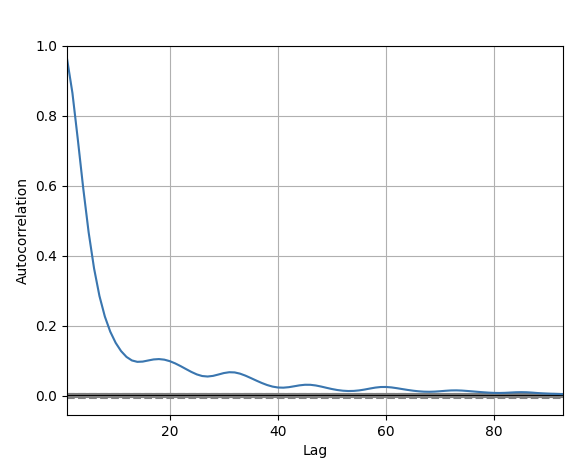
\includegraphics[width=0.6\textwidth]{auto_correlation.png}
\caption{Autocorrelation shows how much the data is correlated with itself at different time lags}
\end{figure}

A significant drop of occurs at around lag 10-15, which  makes $chunk\_len$ set to 10 a good value. Furthermore the function splits the training data into a list of separate, trainable sequences, where each individual sequence has a label(the next value to predict) associated with it. These data sequences are later split into a training and testing set with a 99/1 ratio. 

\subsection{Setting up the RNN}

The \texttt{LSTM\_RNN} class defines a RNN network based on PyTorch's \texttt{nn.Module}:

\begin{lstlisting}
import torch
import torch.nn as nn
from device import device as default_device

class LSTM_RNN(nn.Module):
    def __init__(self, input_size, hidden_size, output_size, num_layers=1, device=default_device):
        """
        input_size: input feature size, in this case 3 for the Lorenz system
        output_size: output feature size, in this case 3 for the Lorenz system
        hidden_size: number of hidden units in the LSTM
        """
        super(LSTM_RNN, self).__init__()
        self.hidden_size = hidden_size
        self.num_layers = num_layers

        self.lstm = nn.LSTM(
            input_size, hidden_size, num_layers=num_layers, batch_first=True
        )
        self.output_activation = nn.Linear(hidden_size, output_size)
        self.device = device

    def forward(self, inputSeq):
        # inputSeq shape [batch_size, seq_len, feature_size]
        batch_size = inputSeq.size(0)
        state = self.init_state(batch_size)
        lstm_out, _ = self.lstm(inputSeq, state)

        # Select the last point in the sequence
        prediction = self.output_activation(lstm_out[:, -1, :])

        return prediction

    def init_state(self, batch_size):
        # Initializing the hidden and cell states for the LSTM based on the batch size
        state = (
            torch.zeros(self.num_layers, batch_size, self.hidden_size).to(self.device),
            torch.zeros(self.num_layers, batch_size, self.hidden_size).to(self.device),
        )
        return state
\end{lstlisting}

\texttt{input\_size} is the dimensionality of the input vector(in this case three for the x, y and z values). The constructor initializes the LSTM layer and output activation layer. The \texttt{forward} method is passing the input through the torhc.nn.LSTM cell and the activation layer to compute the output. The \texttt{init\_state} method initializes the LSTM's internal state with zeros for each new batch. \\

The model is then instantiated like this:
\begin{lstlisting}
from get_training_data import x_train, y_train
from lstm_rnn import LSTM_RNN
from torch import nn
from torch.utils.data import DataLoader, TensorDataset
import torch.optim as optim
import torch
from torch.optim.lr_scheduler import ExponentialLR
import optuna
from device import device as default_device

def train_rnn_lstm(
    hidden_size=32,
    num_layers=1,
    learning_rate=0.0005,
    batch_size=32,
    epochs=5,
    gamma=0.8,
    trial = None,
    device=default_device,
):
    x_train_device = x_train.to(device)
    y_train_device = y_train.to(device)

    train_data = TensorDataset(x_train_device, y_train_device)
    train_dataloader = DataLoader(train_data, batch_size=batch_size)

    input_size = x_train_device.shape[2]
    output_size = y_train_device.shape[1]
    model = LSTM_RNN(input_size, hidden_size, output_size, num_layers, device).to(device)

    loss_fn = nn.MSELoss()
    optimizer = optim.Adam(model.parameters(), lr=learning_rate)
    scheduler = ExponentialLR(optimizer, gamma=gamma)
\end{lstlisting}

 It uses mean squared error loss function and the adam optimizer. It also uses an exponentially decaying learning step scheduler, which has proven great for manaing learning rate at many epochs. \\ \\  The RNN network is later on trained with the following training loop:

\begin{lstlisting}
def train(dataloader, model, loss_fn, optimizer):
    size = len(dataloader.dataset)
    num_batches = len(dataloader)
    model.train()
    running_loss = 0.0

    for batch_nbr, (seq, label) in enumerate(dataloader):
        seq, label = seq.to(device), label.to(device)
        label = label.squeeze(1) # Remove the extra middle dimension, in this case label shape is [batch_size, 1, feature_size]
        prediction = model(seq)
        loss = loss_fn(prediction, label)

        optimizer.zero_grad()
        loss.backward()
        optimizer.step()

        running_loss += loss.item()
        if batch_nbr % 100 == 0:
            current = batch_nbr * len(seq)
            print(f"loss: {loss:>7f}  [{current:>5d}/{size:>5d}]")

    running_loss /= num_batches
    print(f"Average loss for epoch: {running_loss:>7f}")
    return running_loss

epochs = 5
for t in range(epochs):
    print(f"epoch {t + 1} \n--------------")
    train(train_dataloader, model, loss_fn, optimizer)
    if trial is not None:
        trial.report(loss, t)
        if trial.should_prune():
            raise optuna.exceptions.TrialPruned()

    scheduler.step()
print("Done")
torch.save(model.state_dict(), 'lstm_rnn_lorenz.path')
\end{lstlisting}
The training loop iterates over the dataset, feeding batches of data to the model, calculating the loss, and updating the model parameters through backpropagation. Finally after five epochs, the model's parameters are saved.

\subsection{Setting up the transformers architecture}

The transfomers class is written as follows:

\begin{lstlisting}
import math
import torch
from torch import nn, Tensor
from torch.nn import TransformerEncoder, TransformerEncoderLayer

class TransformerModel(nn.Module):
    def __init__(self, ntoken: int, d_model: int, nhead: int, d_hid: int, nlayers: int, dropout: float = 0.5):
        """
        ntoken: The size of the vocabulary (total number of unique tokens).
        d_model: The dimensionality of the token embeddings (the size of the vectors that represent each token).
        nhead: The number of attention heads in the multi-head attention mechanisms.
        d_hid: The dimensionality of the feedforward network model in the transformer encoder.
        nlayers: The number of sub-encoder-layers in the transformer encoder.
        dropout: The dropout rate, a regularization technique to prevent overfitting.


        """
        super().__init__()
        self.model_type = 'Transformer'
        self.pos_encoder = PositionalEncoding(d_model, dropout)
        encoder_layers = TransformerEncoderLayer(d_model, nhead, d_hid, dropout, batch_first=True)
        self.transformer_encoder = TransformerEncoder(encoder_layers, nlayers)
        ##Use linear layer instead of traidiontal embedding layer due to continous data
        self.input_linear = nn.Linear(3, d_model)
        self.d_model = d_model
        self.output_linear = nn.Linear(d_model, 3)

        self.init_weights()

    def init_weights(self) -> None:
        initrange = 0.1
        self.input_linear.weight.data.uniform_(-initrange, initrange)
        self.input_linear.bias.data.zero_()
        self.output_linear.bias.data.zero_()
        self.output_linear.weight.data.uniform_(-initrange, initrange)

    def forward(self, src: Tensor) -> Tensor:
        """
        Arguments:
            src: Tensor, shape ``[seq_len, batch_size]``
            src_mask: Tensor, shape ``[seq_len, seq_len]``

        Returns:
            output Tensor of shape ``[seq_len, batch_size, ntoken]``
        """
        src = self.input_linear(src) * math.sqrt(self.d_model)
        src = self.pos_encoder(src)
        output = self.transformer_encoder(src)
        output = self.output_linear(output)
        return output
    
\end{lstlisting}

This transformers class utilizes the inbuild TransofrmerEncoder and TransformerEncoderLayer built into pytorch. The input is first passed through a linear layer to transform the input data into the d\_model dimensionality. The input is then passed through a positional encoding layer to add information about the position of the tokens in the sequence. The output is then passed through the transformer encoder and then through a linear layer to transform the output back to the original dimensionality. The positional encoding is defined as:

\begin{lstlisting}
class PositionalEncoding(nn.Module):
    def __init__(self, d_model: int, dropout: float = 0.1, max_len: int = 5000):
        super().__init__()
        self.dropout = nn.Dropout(p=dropout)

        position = torch.arange(max_len).unsqueeze(1)
        div_term = torch.exp(torch.arange(0, d_model, 2) * (-math.log(10000.0) / d_model))
        pe = torch.zeros(max_len, 1, d_model)
        pe[:, 0, 0::2] = torch.sin(position * div_term)
        pe[:, 0, 1::2] = torch.cos(position * div_term)
        self.register_buffer('pe', pe)

    def forward(self, x) :
        """
        Arguments:
            x: Tensor, shape ``[seq_len, batch_size, embedding_dim]``
        """
        x = x + self.pe[:x.size(0)]
        return self.dropout(x)
\end{lstlisting}

The positional encoding is a sine and cosine function of different frequencies that are added to the input data. This is to give the network information about the position of the tokens in the sequence. The frequencies are chosen to be logarithmically spaced. \\ \\ The model is then trained in a similar fashion to the RNN model.

\begin{lstlisting}
def train_transformer(
    hidden_dim=500,
    nhead=2,
    num_layers=2,
    learning_rate=0.0005,
    batch_size=8,
    d_model=128,
    dropout=0.1,
    epochs=5,
    trial= None,
    device=default_device
):
    assert (
        d_model % 2 == 0
    ), "d_model must be an even number! This is due to how positional encoding is implemented."

    x_train_device = x_train.to(device)
    y_train_device = y_train.to(device)

    train_data = TensorDataset(x_train_device, y_train_device)
    train_dataloader = DataLoader(train_data, batch_size=batch_size)

    model = TransformerModel(
        d_model=d_model,
        nhead=nhead,
        d_hid=hidden_dim,
        nlayers=num_layers,
        dropout=dropout,
    ).to(device)

    loss_fn = nn.MSELoss()
    optimizer = optim.Adam(model.parameters(), lr=learning_rate)
    scheduler = ExponentialLR(optimizer, gamma=0.9)
\end{lstlisting}

It also uses the same training loop.

\subsection{Setting up the RC-ESN}

\subsection{Training process}
The hyperparameters of the network were optimized using the optuna library implementation of the Tree-structured Parzen Estimator(TPE) algorithm. 

\begin{lstlisting}
    def objective(trial):
    learning_rate = trial.suggest_float("learning_rate", 1e-5, 1e-2)
    batch_size = trial.suggest_categorical("batch_size", [4, 8, 16, 32, 64])
    # epochs = trial.suggest_int('epochs', 5, 10)
    gpu_id = trial.number % 4  
    device = torch.device(f"cuda:{gpu_id}" if torch.cuda.is_available() else default_device)

    if model_type == "Transformer":
        model_hyperparams = {
            "hidden_dim": trial.suggest_categorical(
                "hidden_dim", [256, 512, 768, 1024]
            ),
            "nhead": trial.suggest_int("nhead", 1, 2),
            "num_layers": trial.suggest_int("num_layers", 1, 4),
            "learning_rate": learning_rate,
            "batch_size": batch_size,
            "d_model": trial.suggest_categorical("d_model", [64, 128, 256, 512]),
            "dropout": trial.suggest_float("dropout", 0, 0.4),
            "epochs": 5,
            "trial": trial,
            "device": device,
        }

        model = train_transformer(**model_hyperparams)
        val_loss = evaluate_model(model, device)
        return val_loss

    elif model_type == "RNN_LSTM":
        model_hyperparams = {
            "hidden_size": trial.suggest_categorical(
                "hidden_size", [32, 64, 128, 256, 512]
            ),
            "num_layers": trial.suggest_int("num_layers", 1, 3),
            "learning_rate": learning_rate,
            "batch_size": batch_size,
            "epochs": 5,
            "gamma": trial.suggest_float("gamma", 0.7, 1),
            "trial": trial,
            "device": device,
        }

        model = train_rnn_lstm(**model_hyperparams)
        val_loss = evaluate_model(model, device)
        print(val_loss)
        return val_loss

    elif model_type == "ESN":
        model_hyperparams = {
            "batch_size": batch_size,
            "input_size": 3,
            "output_size": 3,
            "reservoir_hidden_size": trial.suggest_categorical(
                "reservoir_hidden_size", [500, 1000, 1500]
            ),
            "spectral_radius": trial.suggest_float("spectral_radius", 0.5, 1.5),
            "sparsity": trial.suggest_float("sparsity", 0, 0.5),
            "ridge_param": trial.suggest_float("ridge_param", 1e-8, 1e-4),
        }

        model = train_rc_esn(**model_hyperparams)
        val_loss = evaluate_model(model)
        return val_loss

# Optuna study
pruner = optuna.pruners.MedianPruner()
study = optuna.create_study(direction="minimize", pruner=pruner,storage="sqlite:///example_study.db")
study.optimize(
    objective, n_trials=100, n_jobs=4, show_progress_bar=True
)  # n_jobs is number of parallel jobs(one per gpu available)
\end{lstlisting}

It was parallelizad to run on four gpus and took use of purning to preemptively end unpromising trials. Once the best combination of hyperparams was found the networks was retrained over more epochs for optimal results. The optimization took place over 100 trials trained on four RTX 4090s.

\section{Results}
\subsection{RNN}

\begin{figure}[h]
\centering
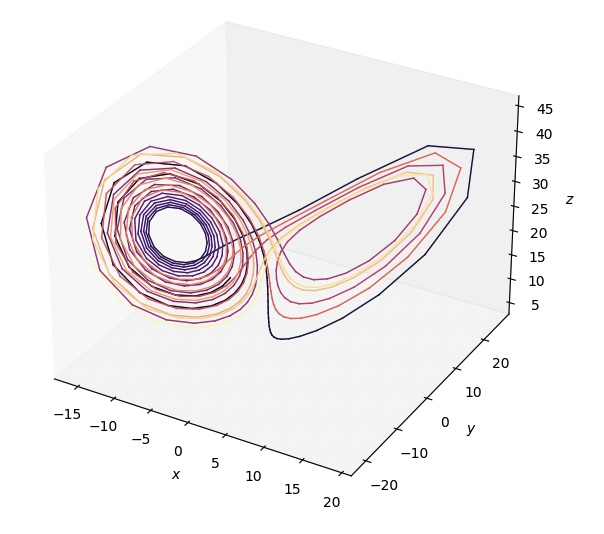
\includegraphics[width=0.6\textwidth]{rnn_lorenz.jpeg}
\caption{RNN Lorenz}
\end{figure}

\begin{figure}[h]
\centering
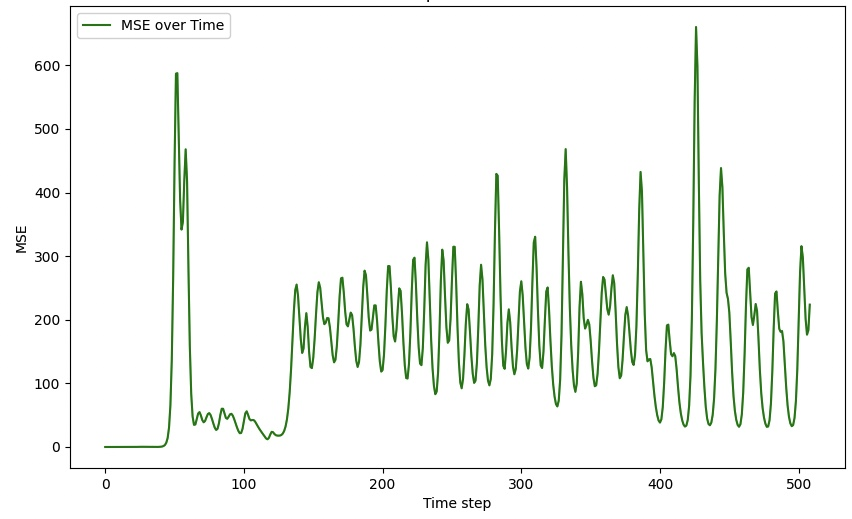
\includegraphics[width=0.6\textwidth]{rnn_mse.jpeg}
\caption{RNN MSE}
\end{figure}

\begin{figure}[h]
\centering
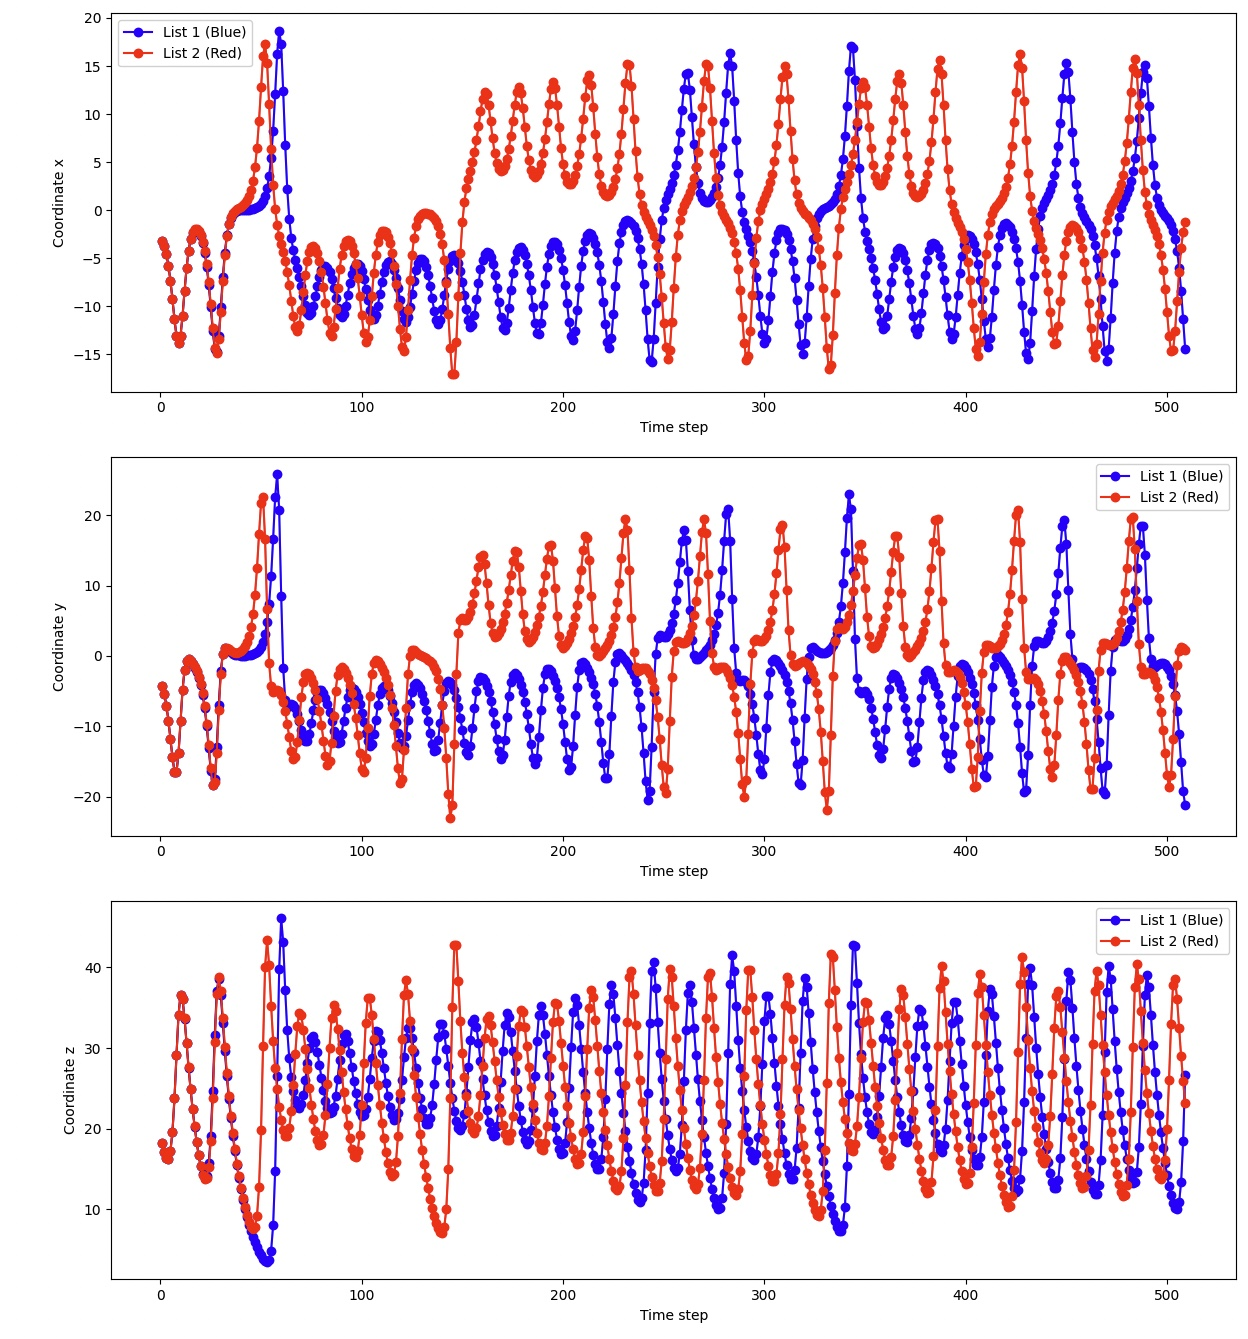
\includegraphics[width=0.6\textwidth]{rnn_path.jpeg}
\caption{RNN path}
\end{figure}

The average MSE for RNN was 50.1579

\subsection{Echos state network}
The average MSE for RNN was 48.7797

\begin{figure}[h]
\centering
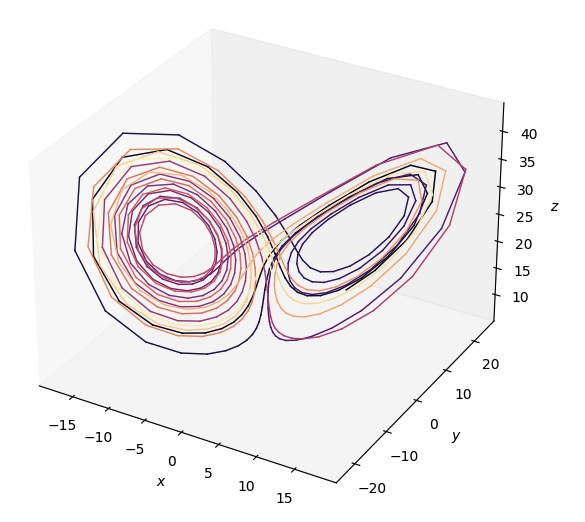
\includegraphics[width=0.6\textwidth]{echo_lorenz.jpeg}
\caption{ESN Lorenz}
\end{figure}

\begin{figure}[h]
\centering
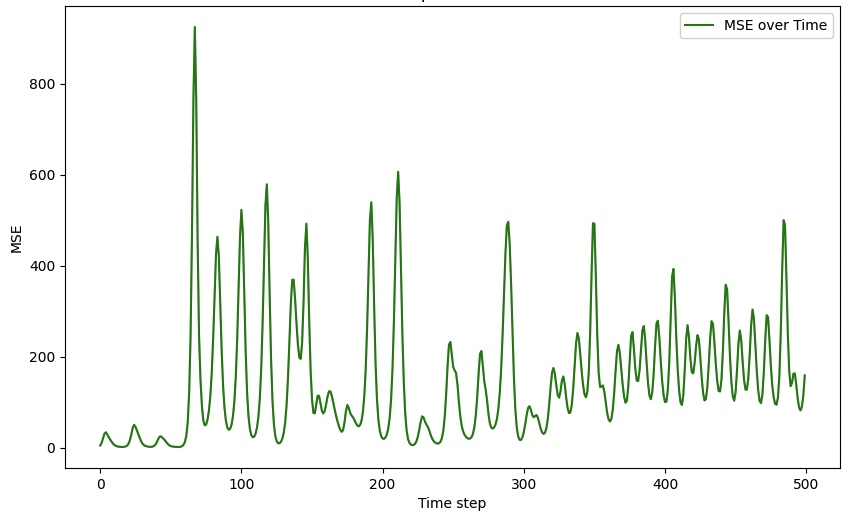
\includegraphics[width=0.6\textwidth]{echo_mse.jpeg}
\caption{ESN MSE}
\end{figure}

\begin{figure}[h]
\centering
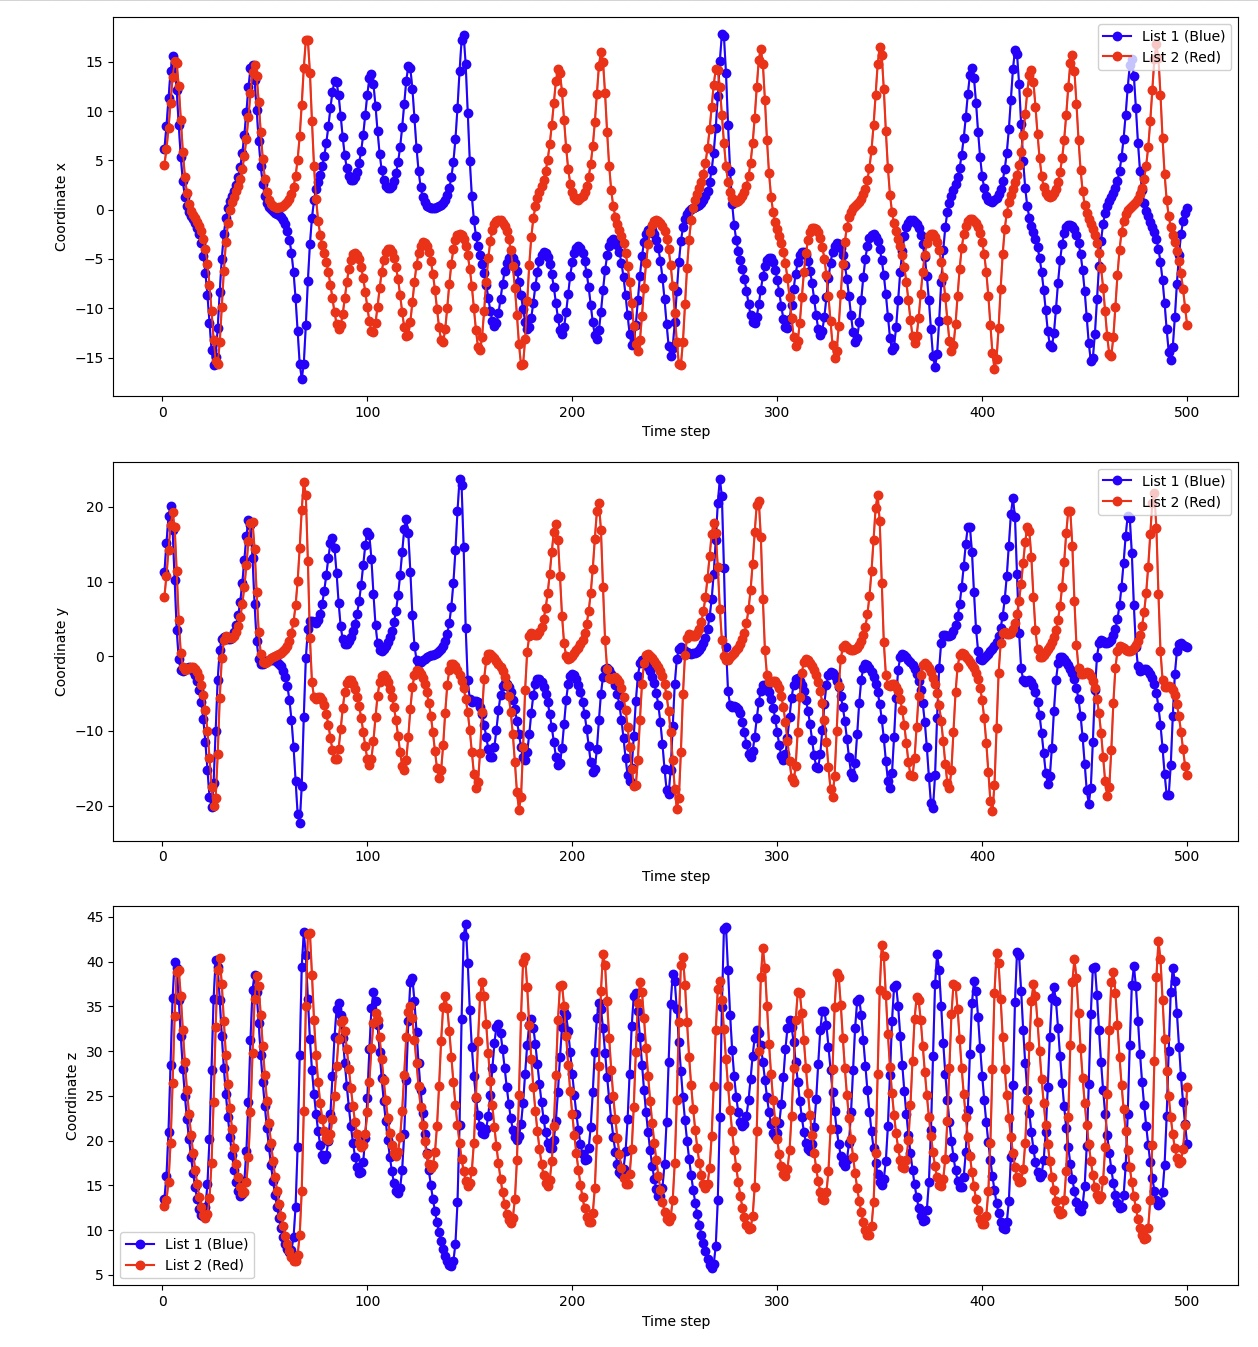
\includegraphics[width=0.6\textwidth]{echo_path.jpeg}
\caption{ESN path}
\end{figure}

\subsection{Transformers}
The average MSE for RNN was 29.1590

\begin{figure}[h]
\centering
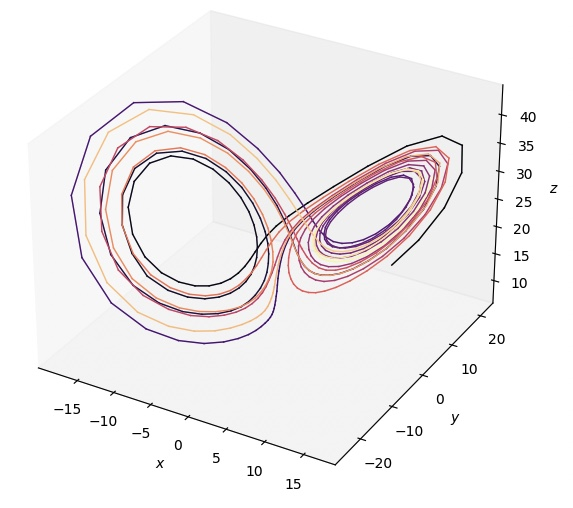
\includegraphics[width=0.6\textwidth]{transformers_lorenz.jpeg}
\caption{Transfomers Lorenz}
\end{figure}

\begin{figure}[h]
\centering
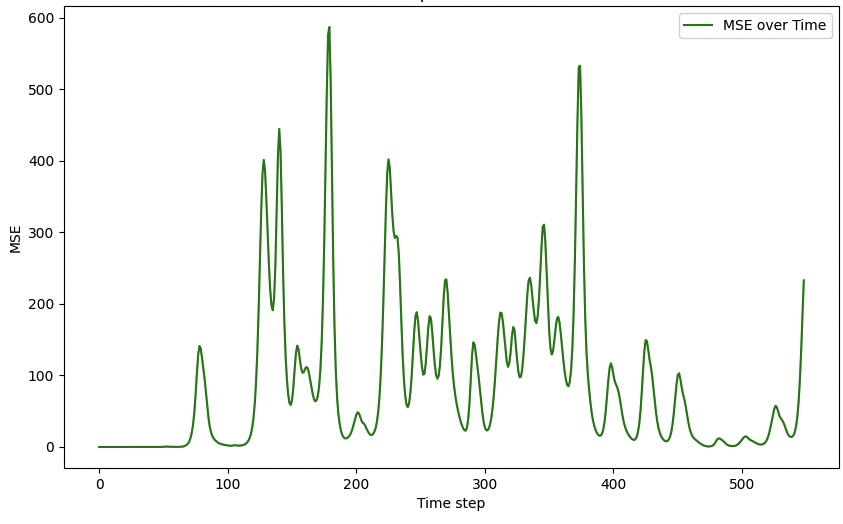
\includegraphics[width=0.6\textwidth]{transformers_mse.jpeg}
\caption{Transformers MSE}
\end{figure}

\begin{figure}[h]
\centering
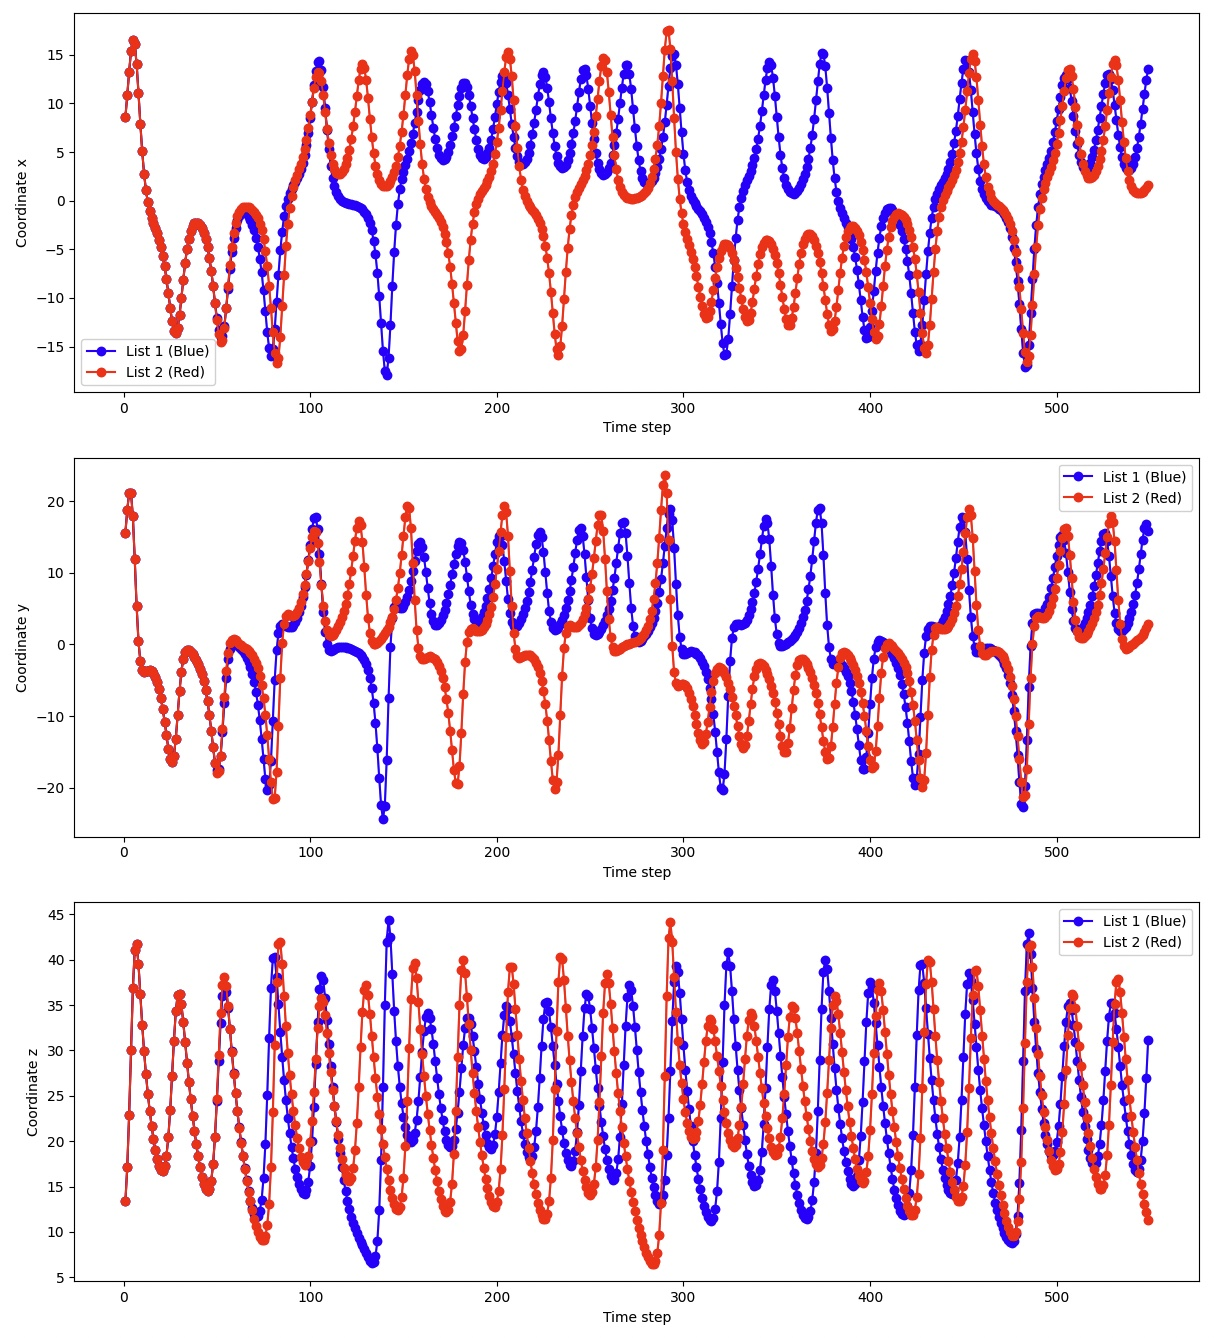
\includegraphics[width=0.6\textwidth]{transformers_path.jpeg}
\caption{Transformers path}
\end{figure}

\bibliographystyle{apalike}
\bibliography{references}

\end{document}

\end{document}
